\section{OlaVM: A Full-featured Zk-friendly ZKVM}\label{sec:ola-vm}
The Zero-knowledge virtual machine(ZKVM) is one of the core modules in OlaVM. It executes the program compiled from the Ola-lang to generates trace tables.The traces are used by ZK prover to construct the ZK proof.
The program format provided from Ola-lang compiler consists of two fields(bytecode and prophets):
\begin{itemize}
    \item \verb|bytecode| consists of instructions and can not be empty.
    \item \verb|prophets| is a array contain all prophets and can be empty.
\end{itemize}

The program snippet is as below:
\begin{lstlisting}[label={lst:program-demo}]
{
  "bytecode": "0x6000080400000000\n0x5\n0x2010000001000000\n0xfffffffeffffffff\n0x4000000840000000\n0x0\n0x0030000001000000\n",
  "prophets": [
    {
      "host": 41,
      "code": "%{\n    entry() {\n        cid.y = sqrt(cid.x);\n    }\n%}",
      "inputs": [
        {
          "name": "cid.x",
          "stored_in": "reg",
          "anchor": "r1",
          "offset": 0
        }
      ],
      "outputs": [
        "cid.y"
      ]
    }
  ]
}
\end{lstlisting}


The ZKVM module contains the following modules:
\begin{itemize}
    \item \verb|design|
    \item \verb|instructions set|
    \item \verb|prophet|
    \item \verb|builtin|
    \item \verb|memory|
    \item \verb|trace generator|
\end{itemize}

\subsection{design}\label{subsec: vm-design}
OlaVM is a virtual machine for the zero-knowledge(ZK) proof.The design principle is ZK friendly and user friendly.
To achieve the targets, designs have been made in the following aspects:

\begin{itemize}
    \item \verb|minimize instructions set|
    \item \verb|use prophet to minimize trace length|
    \item \verb|minimize general register number|
    \item \verb|memory segment|
\end{itemize}

\subsubsection{minimize instructions set}
Every instruction(include builtin instruction) need one column in cpu trace table to present and need different constrains.So the design minimize instructions set to minimize the columns in cpu trace table.
OlaVM use 21 instructions, reference: \ref{table:instruction-set}.

\subsubsection{use prophet to minimize trace length}
There are one application scene: some algorithm is difficult to computation but ease to verify.For example: compute the square root of a radicand.
If implement Newton's method, need many instructions, but by contrast, verify a result is the square root of a radicand is succinct.
ZKVM only need to use the result multiply itself, and verify it is equal to the radicand, only two instructions.
By the second algorithm, how to compute the square root is no matter to ZK circuit and user.
The process of computation is wrapped up in prophet segment and not need to be verified by ZK circuit.
ZK circuit only need to verify the succinct logic $result*result == radicand$.
Use OlaVM to execute two algorithm and generate ZK proof, The second algorithm is 10 times faster than the first traditional algorithm.
reference: \ref{subsec: prophet-interpreter}

\subsubsection{minimize general register number}
Every register need one column in cpu trace table to present and need different constrains.So the design minimize the number of register to minimize the columns in cpu trace table.
OlaVM use 9 general registers and 2 system registers(PC, PSP),  reference: \ref{subsec: zkvm-executor-register}.

\subsubsection{memory segment}
THe memory design is influenced by the prophet.To ensure that the memory trace table can be written by prophet without use instructions,the memory space need be partitioned into several segment.
The prophet segment is write-once for constraint. reference: \ref{subsec: ola-memory}
\subsection{Instruction Set}\label{subsec: instructions-set}

The ZKVM module use instructions and memory addresses to be accessed in the same space.
This is because the ZKVM module has sufficient space for use,
and using a unified space can make the column for storing constraints smaller, reducing overhead.

\subsubsection{register}\label{subsec: zkvm-executor-register}
    Currently, there are two main models for designing the L0 layer of the ZKVM memory hierarchy in the industry, one is the register model and the other is the stack model.
    For the stack model, state updates are implemented according to the first-in-last-out model of the stack. The constraints is relatively simple.
However, the disadvantage is that accessing the state is not user-friendly.
It is not possible to use one instruction to randomly access data at a specific address in the stack. \\
    In contrast, the register model only requires one instruction to complete a randomly read operation, while the stack model requires multiple pop and push operations.
Alternatively, to improve efficiency, swap-like instructions are added in the MidenVM design to optimise randomly access data in the stack.
    For the register model, any register can be randomly accessed.
    However, the disadvantage is that the constraint model requires copy constraints for the upper and lower instructions, and more columns for register selectors.
    Totally, The columns in trace table is lager than the stack model.

    As designed in the last version of whitepaper,OlaVM selects a register model.There are 9 general-purpose registers.
The symbol denote as: $\texttt{r}_0 - \texttt{r}_{8}$.
The $\texttt{r}_{8}$ is used as $\texttt{fp}$(frame pointer). $\texttt{fp}$ is the alias of $\texttt{r}_{8}$.

The PC (program counter) pointer of a loaded program initially points to the instruction at address 0.
As instructions are executed, the value of the address pointed to by the PC changes.
If a jump or call instruction is not executed, the address stored in the PC register is incremented by 1 for each instruction executed, unless the instruction uses an immediate value, in which case the PC is incremented by 2.

The PSP(prophet stack pointer) register is used to alloc the prophet memory segment when ZkVM execute prophet code.In the initial state, set the prophet memory segment start address($2^{64} - 2*2^{32}$) to this register.

\subsubsection{Olavm instructions}\label{subsec: zkvm-executor-instructions}
To minimize the degree of constraints, The ZKVM model use reduced instruction set.

Olavm use Word(64bits) encode instruction.
An instruction is encoded with an opcode and up to three operands, which can be either a register or an immediate value.
An instruction encoding consists of the following 8 fields:
\begin{itemize}
    \item Field1: Field name:NULL.1 bit width,not used.
    \item Field2: Field name:OP1 immediate flag(OP1\_IMM, imm).1-bit width.Set to 0,indicates that A is a register;set to 1, indicates that A is an immediate value.
    \item Field3: Field name:operation0 register(OP0\_REG, reg\_src1).9-bit width.Indicates source op0 register index, index range from 0 to 8.
                  Set to 1 determine operating the register corresponding to the index, otherwise set to 0.
    \item Field4: Field name:operation1 register(OP1\_REG, reg\_src2).9-bit width.Indicates source op1 register index, index range from 0 to 8.
                  Set to 1 determine operating the register corresponding to the index, otherwise set to 0.If all 9 bits set to 0, indicates use PSP(prophet stack pointer) register.
    \item Field5: Field name:destination register(DST\_REG, reg\_dst).9-bit width.Indicates destination register index, index range from 0 to 8.
                  Set to 1 determine operating the register corresponding to the index, otherwise set to 0.
    \item Field6: Field name:opcode selector(opcode\_sel).21-bit width.Indicates the opcode type,set to 1 determine executing the opcode, otherwise set to 0.
    \item Field7: Field name:padding bits(paddings).14-bit width.
                  All bits padding by 0, will be used in the future.
    \item Field8: Field name:immediate data(immediate).This field is option, determined by field2,If filed2 set to 1.
                  This field indicates an immediate value, This field is 2 Word width.
\end{itemize}

The instruction set of the ZkVM model as below, A denoted intermediate or register:
\begin{table}[!ht]
    \resizebox{\textwidth}{!}{%
        \begin{tabular}{|c|c|c|c|c|}
            \hline
            \textit{Type}  & \textit{Instruction} & \textit{Operands} & \textit{Description} & \textit{flag} \\ \hline
            \multirow{2}{*}{Field Operation}  & ADD & ri rj A & Compute rj + A and store the result in ri &   \\ \cline{2-5}
            & MUL & ri rj A & Compute rj * A and store the the result in ri &  \\ \hline
            \multirow{2}{*}{Cmp}  & EQ & ri rj A & Equality comparison and store the the result in ri & rj = A \\ \cline{2-5}
            & NEQ & ri rj A &  check whether rj is not equal A and store the the result in ri & rj != A \\ \cline{2-5}
            & ASSERT & ri  A & Assert ri == A and vm will hang up if assertion fail &  \\  \hline
            Move & MOV & ri A & Copy the data of A to ri &  \\ \hline
            \multirow{5}{*}{Flow} & JMP & A & Set pc equal A &  \\ \cline{2-5}
            & END &  & only appears at the end of the program &  \\  \cline{2-5}
            & CJMP & rj A & If rj = 1, set pc equal A, else increment pc as usual &  \\  \cline{2-5}
            & CALL & A & \multicolumn{1}{l|}{\begin{tabular}[c]{@{}l@{}}The Call instruction consists of the following steps\\ 1. store return pc to the frame address [fp-1].\\ 2. jump to the address A\end{tabular}} &  \\  \cline{2-5}
            & RET &  & \multicolumn{1}{l|}{\begin{tabular}[c]{@{}l@{}}The Ret instruction consists of the following two steps\\ 1. use the memory address stored in the fp register to find the returned pc and jump to the location of the returned pc.\\ 2. update the fp register to the fp before the call\end{tabular}} &  \\ \hline
            \multirow{2}{*}{RAM} & MLOAD & ri [A, imm] & \multicolumn{1}{l|}{\begin{tabular}[c]{@{}l@{}}Read the value from memory [A+imm] and store it into ri. \\ imm is optional, can not represent. \\ A can be a intermediate data or register value.\\ if A is a  register, can follow a immediate data.\end{tabular}}&  \\ \cline{2-5}
            & MSTORE & [A, imm] rj & \multicolumn{1}{l|}{\begin{tabular}[c]{@{}l@{}}Read the value from register rj and store it into memory [A+imm]. \\ imm is optional, can not represent. \\ A can be a intermediate data or register value. \\ if A is a  register, can follow a immediate data.\end{tabular}}&  \\ \hline
            \multirow{8}{*}{BUILTIN} & RANGE CHECK & rj & range check the value in rj  &  \\ \cline{2-5}
            & AND & ri rj A &  Compute rj and A and store the the result in ri &  \\ \cline{2-5}
            & OR & ri rj A &  Compute rj or A and store the the result in ri &  \\ \cline{2-5}
            & XOR & ri rj A &  Compute rj xor A and store the the result in ri &  \\ \cline{2-5}
            & NOT & ri A &  Compute not A and store the the result in ri &  \\ \cline{2-5}
            & GTE & ri rj A &  check whether rj is great than or equal to A and store the the result in ri &  rj >= A \\ \hline
        \end{tabular}%
    }
    \caption{Instruction set}
    \label{table:instruction-set}
\end{table}
\subsection{Memory}\label{subsec: ola-memory}
The memory structure of OlaVM consists of two types(Read-Write and Write-Once) and mapping to disjoint regions of the memory space.
\begin{table}[!ht]
    \resizebox{\textwidth}{!}{
        \begin{tabular}{|c|c|c|}
            \hline
            \textit{Memory Seg}  & \textit{Type} & \textit{Range}  \\ \hline
            random access memory & Read-Write &  $[0,  2^{64}-3\cdot 2^{32}-1] $ \\ \hline
            ecdsa & Write-Once &  $[2^{64}-3\cdot 2^{32}, 2^{64}-2\cdot 2^{32}-1] $ \\ \hline
            poseidon & Write-Once &  [$2^{64}-2\cdot 2^{32},  2^{64}- 2^{32}-1] $ \\ \hline
            prophet & Write-Once &  $[2^{64}-2^{32}, 2^{64}-1]$ \\ \hline
        \end{tabular}}
    \caption{Memory segment range}
    \label{table:memory-segment-range}
\end{table}


OlaVM use B-Tree algorithm to manage the memory address, support random access memory.B-Tree algorithm sort the memory by address and cpu clock when insert data to the memory bu address.
\begin{enumerate}
    \item when random access memory, the time complexity of search is $\texttt{O(logN)}$.
    \item when generate memory trace table by address and clock in ascending order,the memory can direct visit, not need sort again.
\end{enumerate}

The memory structure illustration is as below \ref{fig: B-tree-memory}:
\begin{figure}[!htp]
    \centering
    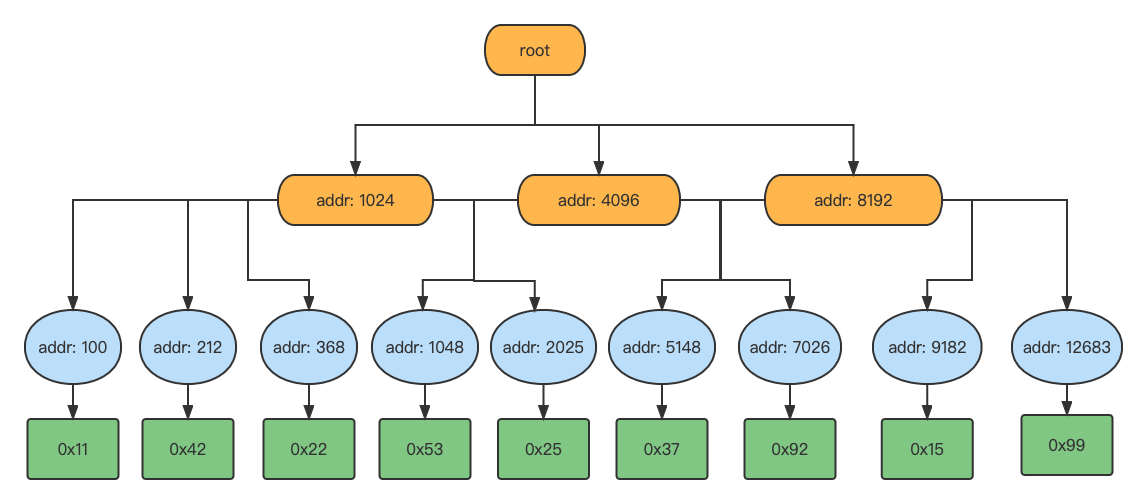
\includegraphics[width=0.8\textwidth]{memory-structure}
    \caption{OlaVM memory structure}
    \label{fig: B-tree-memory}
\end{figure}
\subsection{Prophet Interpreter}\label{subsec: prophet-interpreter}
prophet interpreter runs the prophet code in the field $\texttt{prophets}$ of program.Prophet interpreter does not change the status of PC and $\texttt{r}_{8}$.
It runs the prophet code and stores the status of context id in prophet segment of memory and update the PSP to free prophet memory in ascending order.
The prophet code snippet is as below, the entry procedure is the beginning when prophet interpreter run, the variable with prefix of $\texttt{cid}$ is the context id:
\begin{lstlisting}[label={lst:prophet-demo}]
%{
    function mod(felt x, felt y) -> felt {
        return x % y;
    }

    entry() {
        cid.r = mod(cid.x, cid.y);
    }
%}
\end{lstlisting}

The prophet interpreter illustration is as below.
The pink blocks are the logic relate to prophet interpreter.
The blue blocks are the logic relate to OlaVM executor.
The green blocks are the begin and end.
Prophet interpreter is embedded to OlaVMv executor as a module.
\ref{fig: prophet-interpreter-logic}:
\begin{figure}[!htp]
    \centering
    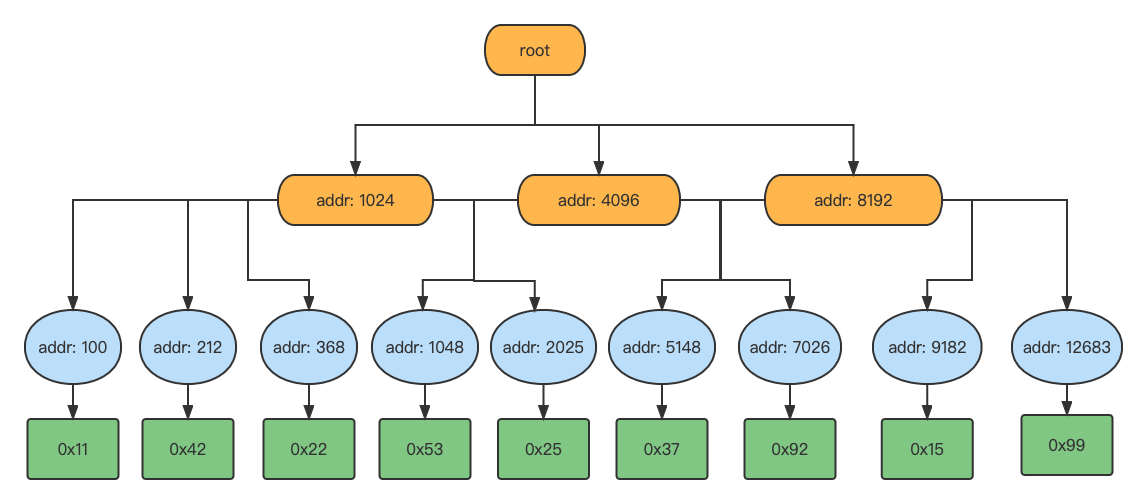
\includegraphics[width=0.8\textwidth]{memory-structure}
    \caption{OlaVM prophet interpreter flow}
    \label{fig: prophet-interpreter-logic}
\end{figure}

\subsection{builtin}\label{subsec: instructions-builtin}
OlaVM implement builtin to support range check, hash, etc.Builtin code need be encoded in instruction set,the definition in builtin rows of table \ref{table:instruction-set}.

\subsubsection{range check}
Range check builtin is used to check u32 type data.OlaVM put check data into range check trace table when execting the range check builtin.

\subsubsection{bitwise}
Bitwise builtin is used to implement the and, or, xor three bitwise operations of u32 type data.OlaVM run the builtin logic and put operation result into bitwise trace table.
Meanwile, put two source operands into range check trace table.

\subsubsection{comparison}
Comparison builtin is used to implement gte(great or equal) comparison. OlaVM run the builtin logic and operation result into comparison trace table.
Meanwile, put two source operands into range check trace table.
